\begin{figure}
  \center
  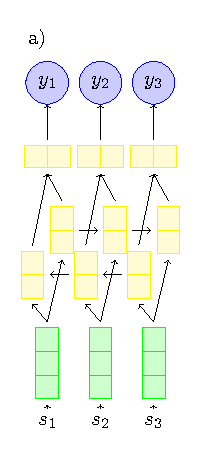
\includegraphics[scale=.45]{figures/rnnextractor.pdf}
  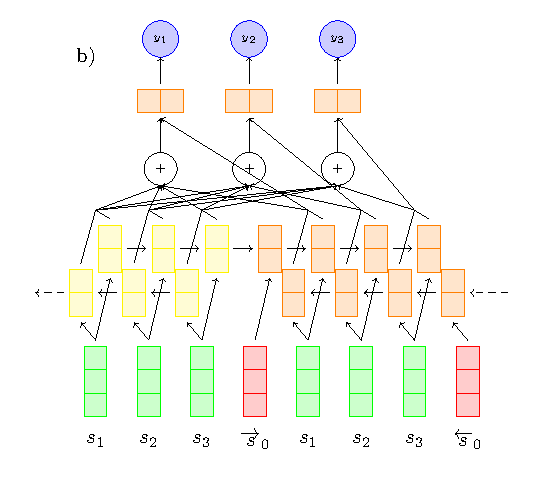
\includegraphics[scale=.45]{figures/s2s_extractor.pdf}
  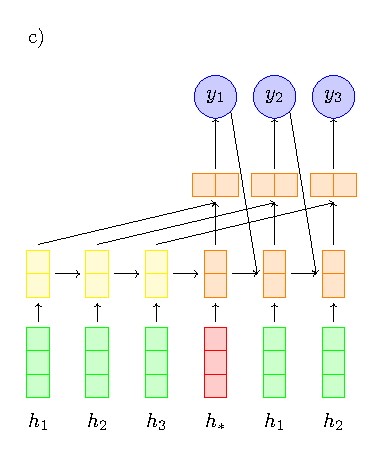
\includegraphics[scale=.45]{figures/clextractor.pdf}
  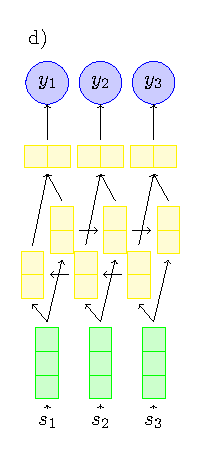
\includegraphics[scale=.45]{figures/sr_extractor.pdf}
  \caption{Sentence extractor architectures: a) RNN, b) Seq2Seq,
  c) Cheng \& Lapata, and d) SummaRunner. The $\bigoplus$ indicates 
  attention. Green repesents sentence encoder output, yellow and orange
  indicates
  extractor encoder and decoder hidden states respectively, and red indicates
  learned ``begin decoding'' embeddings. }
  \label{fig:extractors}
\end{figure}




The goal of extractive text summarization is to select a subset of a 
document's text to use as a summary, i.e. a short gist or excerpt of the 
central content.
Typically, we impose a budget on the length of the summary in either 
words or bytes. In this work, we focus on \textit{sentence} extractive 
summarization, 
where the basic unit of extraction is a sentence and impose a word limit as 
the budget.

We model the sentence extraction task as a sequence tagging problem, 
following \cite{conroy2001text}. 
Specifically, given a document containing $\docSize$ sentences 
$\sent_1, \ldots, \sent_{\docSize}$ we generate a summary by predicting a 
corresponding label sequence $\slabel_1, \ldots, \slabel_{\docSize} 
\in \{0, 1\}^{\docSize}$, where $\slabel_i = 1$ 
indicates the $i$-th sentence is to be included in the summary.
Each sentence is itself a sequence of word embeddings 
$\sent[i] = \wordEmb[1]^{(i)}, \ldots, \wordEmb[{|\sent[i]|}]^{(i)}$ where
$|\sent[i]|$ is the length of the sentence in words.
The word budget $c \in \mathbb{N}$ 
enforces a constraint that the total summary word length 
$\sum_{i=1}^\docSize \slabel_i \cdot |\sent[i]| \le c$.






%\hal{maybe introduce some more notation here, like $s$ is a sequence of $w$s, etc. i think that might be all you need.}


For a typical deep learning model of extractive 
summarization there are two main design decisions:
%At a high level, all the models considered in this paper share the same two part structure: 
\textit{a)}  the choice of \textit{sentence encoder} 
which maps each sentence \sent[i] 
%(treated as a sequence of word embeddings) 
to an embedding $\sentEmb[i]$, 
%\hal{notation class, you used $d$ already for number of sentences} 
and 
\textit{b)} the choice of \textit{sentence extractor} 
which maps a sequence of sentence embeddings 
$\sentEmb = \sentEmb[1],\ldots, \sentEmb[\docSize]$  
to a sequence of extraction
decisions $\slabel = \slabel_1,\ldots,\slabel_{\docSize}$.
%and predicts which sentences to extract to produce the 
%extract summary. 









% anchor
\subsection{Sentence Encoders} \label{sec:senc}
\begin{figure}
  \center
  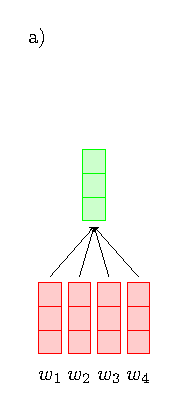
\includegraphics[scale=.7]{figures/avgsentencoder.pdf}
  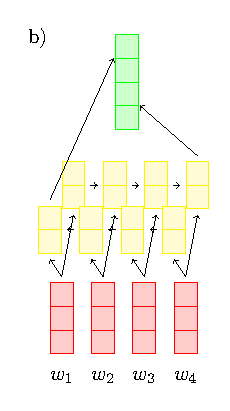
\includegraphics[scale=.7]{figures/rnnsentencoder.pdf}
  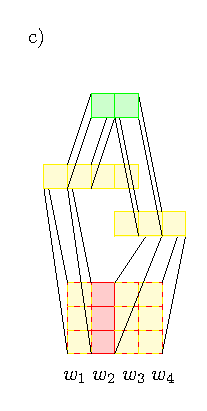
\includegraphics[scale=.7]{figures/cnnsentencoder.pdf}
  \caption{Sentence encoder architectures: a) averaging encoder, b) RNN encoder
           c) CNN encoder. Red indicates word embeddings, yellow indicates
           RNN hidden states or convolutional activations, and green 
           indicates the sentence embedding that is passed to the extractor
           module.}
    \label{fig:encoders}
\end{figure}

We treat each sentence $\sent = \{\wemb_1, \ldots, \wemb_{|\sent|}\}$ 
as a sequence of word embeddings, where $|\sent|$ is the total number of words
in the sentence. We experiment with three architectures for mapping sequences
of word embeddings to a fixed length vector: average pooling, RNNs, and CNNs.
See Figure~\ref{fig:encoders} for a diagram of the three encoders.

\textbf{Averaging Encoder} The averaging encoder (\textit{AVG}) is the simplest
method and has the added benfit of being parameter free. 
A sentence encoding is simply the average of its word embeddings: 
$\operatorname{enc}(\sent) = \frac{1}{|\sent|} \sum_{\wemb \in \sent} \wemb$.


\textbf{RNN Encoder} The \textit{RNN} sentence encoder uses the concatenation 
of the
final output states of a forward and backward RNN over the sentence's word
embeddings. We use a Gated Recurrent Unit (GRU) \cite{cho} for the RNN cell,
since it has fewer parameters than the equivalent LSTM but with similar 
performance. Formally, an \textit{RNN} sentence encoding is defined as
$\operatorname{enc}(s) = [\rSentVec_{|\sent|}; \lSentVec_1]$
where 
\begin{align} 
\rSentVec_i &= \rgru(w_i, \rSentVec_{i-1}) \\
\lSentVec_i &= \lgru(w_i, \lSentVec_{i+1}) 
\end{align}
for all $i \in 1, \ldots, |\sent|$. $\rgru$ amd $\lgru$ indicate the 
forward and backward GRUs respectively, and each have separate learned 
parameters.
The initial states $\rSentVec_0$ and $\lSentVec_{\sentSize + 1}$ are not 
learned and are set to zero vectors.

\textbf{CNN Encoder} The \textit{CNN} sentence encoder uses a series of 
convolutional feature maps to encode each sentence. This encoder is similar
to the convolutional architecture of \cite{kim} used for text classification
tasks and performs a series of ``one-dimensional'' convolutions over 
word embeddings. 
The \textit{CNN} encoder has hyperparameters
associated with the window sizes $\maxWindowSize \subset \mathcal{N}$ of the convolutional filter 
(i.e. the number of words associated with each convolution) and the number of 
feature maps $\maxFeatureMaps$ associated with each filter
(i.e. the output dimension of each 
convolution). 
The \textit{CNN} sentence encoding is computed as follows:
\begin{align}
 \specActivation_i &= \specConvBias 
    + \sum^\filterWindowSize_{j=1} \specConvWeight_j \cdot \wemb_{i + j -1}\\
  \specFeatureMap &= \max_{i\in 1,\dots, |\sent| - \filterWindowSize + 1} 
                      \relu\left(\specActivation_i\right) \\
 \senc(s) &= \left[\specFeatureMap | 
   \numFeatureMaps \in \{1, \ldots, \maxFeatureMaps\},
   \filterWindowSize \in \maxWindowSize
   \right]
\end{align}
where $\specConvBias\in\mathcal{R}$ and $\specConvWeight \in 
\mathcal{R}^{\filterWindowSize \times \wembdim}$ are learned bias and filter
weight parameters respectively, and $\relu(x) = \max(0, x)$ is the rectified
linear unit \cite{relu}.





\subsection{Sentence Extractors} \label{sec:sext}



Sentence extractors take sentence embeddings $h_{1:n}$ and produce an extract $y_{1:n}$.
The sentence extractor is essentially a discriminative 
classifier $p(\slabel_{1:n} | \sentEmb_{1:n})$.
Previous neural network approaches to sentence extraction have assumed 
an auto-regressive model, leading to a semi-Markovian
factorization of the extractor probabilities 
$p(\slabel_{1:n}|\sentEmb)=\prod_{i=1}^\docSize 
p(\slabel[i]|\slabel[<i],\sentEmb)$,
where each prediction \slabel[i] is dependent on \emph{all} 
previous \slabel[j] for
all $j < i$. We compare two such models proposed by \citet{cheng2016neural}
and \citet{nallapati2017summarunner}.
A simpler approach that does not allow interaction among the $y_{1:n}$
is to 
%\hal{a simpler approach (explain why simpler) is a fully factored representation 
  model $p(\slabel_{1:n}|\sentEmb) = \prod_{i=1}^n p(y_i|h)$, 
  which we explore in two proposed extractor models the we refer to as the RNN 
  and Seq2Seq extractors.
Implementation details for all extractors are in Appendix~\ref{app:sentextractors}.


\paragraph{Previously Proposed Sentence Extractors}
 We consider two recent state-of-the-art extractors.
%\hal{if you're hurting for space, you could probably describe these both in one paragraph, leaving off the stuff about what they use as encoders, etc., and really just making the point that they use $y<i$ to predict $yi$}

%\paragraph{Cheng \& Lapata Extractor} 
 The first, proposed by 
\citet{cheng2016neural}, %, which we refer to as the Cheng \& Lapata Extractor,
is built around a sequence-to-sequence model.
First, each sentence embedding\footnote{\citet{cheng2016neural} used an CNN sentence encoder with 
this extractor architecture; in this work we pair the Cheng \& Lapata extractor
with several different encoders.} is
fed into an encoder side RNN, with the final encoder state passed to the
first step of the decoder RNN. On the decoder side, the same sentence 
embeddings are fed as input to the decoder and decoder outputs are used to
predict each $y_i$. The decoder input is weighted by the previous extraction
probability, inducing the dependence of $y_i$ on $y_{<i}$.
See \autoref{fig:extractors}.c for a graphical layout of the extractor
and Appendix~\ref{app:clextractor} for details.

%?, but are delayed by one step and 
%?weighted by their prediction probability, i.e. at decoder step $t$,
%?$p(\slabel[t-1]|\slabel[<t-1], \sentEmb[<t-1]) \cdot \sentEmb[t-1]$\hal{why did you switch from $i$ to $t$?}
%?is fed into the decoder\hal{i don't udnerstand what this means. what op is $\cdot$?}. The decoder output at step $t$ is concatenated 
%?to the encoder output step $t$ and fed through a multi-layer perceptron
%?with one hidden layer and sigmoid unit output computing the $t$-th
%?extraction probability $p(\slabel[t]|\slabel[<t], \sentEmb[<t])$. \textcolor{red}{See Figure 2.c. for a graphical view. Full model details are presented in ??}.
%?

\citet{nallapati2017summarunner} proposed
a sentence extractor, which we refer to as the SummaRunner Extractor,
that factorizes the extraction probability into contributions 
from different sources.
First, a bidirectional RNN is run over the sentence embeddings\footnote{\citet{nallapati2017summarunner}
    use an RNN sentence encoder with 
this extractor architecture; in this work we pair the SummaRunner extractor
with different encoders. } and the output
concatenated. A representation of the whole document is made by 
averaging the RNN output. A summary representation is also constructed 
by taking the sum of the previous RNN outputs weighted by their extraction
probabilities. Extraction predictions are made using 
the RNN output at the $i$-th step, the document representation, and 
$i$-th version of the summary representation, along with factors for 
sentence location in the document. The use of the iteratively constructed
summary representation creates a dependence of $y_i$ on all $y_{<i}$.
See \autoref{fig:extractors}.d for a graphical layout,
and Appendix~\ref{app:srextractor} for details.

%?A document representation $q$ is created by passing the 
%?averaged RNN output through a fully connected layer.
%?
%?Given the RNN output $z_t$ at the step $t$, the following scores are created:
%?\begin{enumerate}[nolistsep,noitemsep]
%?\item a content score $W^{(con)}z_t$,
%?\item a salience score $z_t^TW^{(sal)}q$,
%?\item a novely score $-z_t^TW^{(nov)}\tanh(g_t)$,
%?\end{enumerate}
%?where $g_t = \sum_{i=1}^{t-1} p(y_i=1|y_{<i}, h_{<i}) \cdot z_i$.
%?These scores are summed along with a bias term and a bias for sentence 
%?position and the quarter of the document\hal{what does ``the quarter of the document'' mean? sentence position quartile?} and fed through a sigmoid activation
%?to compute $p(y_t=1|y_{<t}, h_{<t})$.


\paragraph{Proposed Sentence Extractors}
We propose two sentence extractor models that 
make a stronger conditional independence 
assumption $p(\slabel|\sentEmb)=\prod_{i=1}^\docSize p(\slabel[i]|\sentEmb)$,
essentially making independent predictions conditioned on $\sentEmb$.
%In theory, our models should \hal{why should they?} perform worse because of this, however, as
%we later show, this is not the case empirically.

\paragraph{RNN Extractor}
    Our first proposed model is a very simple bidirectional
RNN based tagging model. As in the RNN sentence encoder we use a GRU cell.
The forward and backward outputs of each sentence are passed through a 
multi-layer perceptron with a logsitic sigmoid output 
to predict the probability
of extracting each sentence. 
See \autoref{fig:extractors}.a for a graphical layout,
and Appendix~\ref{app:rnnextractor} for details.


\paragraph{\sts~Extractor} One shortcoming of the RNN extractor is that long range
information from one end of the document may not easily be able to affect 
extraction probabilities of sentences at the other end. 
Our second proposed model, the \sts~extractor mitigates this problem with an 
attention 
mechanism commonly
used for neural machine translation \cite{bahdanau2014neural} and 
abstractive summarization \cite{see2017get}. 
The sentence embeddings are first
encoded by a bidirectional $\gru$. A separate decoder $\gru$ transforms each 
sentence into a query vector which attends to the encoder output. The
attention weighted encoder output and the decoder $\gru$ output are concatenated
and fed into a multi-layer percepron to compute the extraction probability.
See \autoref{fig:extractors}.b for a graphical layout,
and Appendix~\ref{app:s2sextractor} for details.

%
%We study three architectures for the sentence encoders, namely, 
%embedding averaging, RNNs, and 
%CNNs.
%We also propose two simple models for the sentence extractor and compare
%to the previously proposed extractors of 
%\citet{cheng2016neural} and \citet{nallapati2017summarunner}.
%\hal{i think it's still confusing what's new and what's not. maybe you can somewhat mark? like things with $\star$ are new and ones without are old or something?}
%The prior works differ significantly but make the same semi-Markovian
%factorization of the extraction decisions, i.e. 
%$p(\slabel|\sentEmb)=\prod_{i=1}^\docSize p(\slabel[i]|\slabel[<i],\sentEmb)$,
%where each prediction \slabel[i] is dependent on all previous \slabel[j] for
%all $j < i$.
%By contrast, our extractors make a stronger conditional independence 
%assumption $p(\slabel|\sentEmb)=\prod_{i=1}^\docSize p(\slabel[i]|\sentEmb)$,
%essentially making independent predictions conditioned on $\sentEmb$.
%In theory, our models should perform worse because of this, however, as
%we later show, this is not the case empirically.
%
%
%
%\hal{i think you might need a subsection at the end of this section with oen or two paragraphs of compare/contrast the different models, esp if details are going to appendix}
%




%%% Local Variables:
%%% mode: latex
%%% TeX-master: "dlextsum.emnlp18"
%%% End:
